\documentclass[11pt]{article}
\usepackage[utf8]{inputenc}	% Para caracteres en español
\usepackage{amsmath,amsthm,amsfonts,amssymb,amscd}
\usepackage{multirow,booktabs}
\usepackage[table]{xcolor}
\usepackage{fullpage}
\usepackage{lastpage}
\usepackage{enumitem}
\usepackage{fancyhdr}
\usepackage{mathrsfs}
\usepackage{wrapfig}
\usepackage{setspace}
\usepackage{calc}
\usepackage{multicol}
\usepackage{cancel}
\usepackage{float}
\usepackage{physics}
\usepackage[retainorgcmds]{IEEEtrantools}
\usepackage[margin=1cm]{geometry}
\usepackage{amsmath}
\newlength{\tabcont}
\setlength{\parindent}{0.0in}
\setlength{\parskip}{0.05in}
\usepackage{empheq}
\usepackage{framed}
\usepackage[most]{tcolorbox}
\usepackage{xcolor}
\usepackage[version=3]{mhchem}
\usepackage[english]{babel}
\usepackage[utf8]{inputenc}
\usepackage{graphicx}
\usepackage[colorinlistoftodos]{todonotes}
\usepackage{mdframed}

\colorlet{shadecolor}{orange!15}
\parindent 0in
\parskip 12pt
\geometry{margin=1in, headsep=0.25in}
\theoremstyle{definition}
\newtheorem{defn}{Definition}
\newtheorem{reg}{Rule}
\newtheorem{exer}{Exercise}
\newtheorem{note}{Note}
\begin{document}
\setcounter{section}{2}
%\setcounter{subsection}{}
\title{Problem Set 6}

%==============================================================
%\thispagestyle{empty}
\pagestyle{fancy}
\fancyhf{}
\rhead{Physics 180}
\chead{Problem Set 6}
\lhead{Olyn D. Desabelle}
\rfoot{Page \thepage}

\begin{center}
{\LARGE \bf Problem Set 6}\\
%{\large Physics 180}\\
%Olyn D. Desabelle
\end{center}

\begin{figure}[h!]
    \centering
    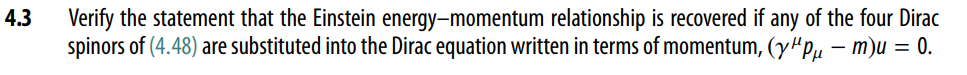
\includegraphics[scale = 0.5]{4.3.png}
\end{figure}

The Dirac equation reads:

\begin{align}
    (\gamma^{\mu} p_{\mu} - m)u = 0
\end{align}

working back and substituting corresponding $\mu$ for the spinors (from Equations 4.40-4.41 of Thomson):

\begin{align}\label{expanded dirac}
    (\gamma^{0} E - \gamma^{1} p_{x} - \gamma^{2} p_{y} - \gamma^{3} p_{z} - m) u(E,\mathbf{p}) e^{i(\mathbf{p}\cdot\mathbf{x} - Et)}  = 0
\end{align}

we have the following matrix expressions for $\gamma$ (from Equation 4.35 of Thomson):

\begin{align*}
    \gamma^{0} = 
    \begin{pmatrix}
        1&0&0&0\\ 
        0&1&0&0\\ 
        0&0&-1&0\\ 
        0&0&0&-1
    \end{pmatrix}
    \;\;\;
    \gamma^{1} = 
    \begin{pmatrix}
        0&0&0&1\\ 
        0&0&1&0\\ 
        0&-1&0&0\\ 
        -1&0&0&0
    \end{pmatrix}\\
    \gamma^{2} = 
    \begin{pmatrix}
        0&0&0&-i\\ 
        0&0&i&0\\ 
        0&i&0&0\\ 
        -i&0&0&0
    \end{pmatrix}
    \;\;\;
    \gamma^{3} = 
    \begin{pmatrix}
        0&0&1&0\\ 
        0&0&0&-1\\ 
        -1&0&0&0\\ 
        0&1&0&0
    \end{pmatrix}
\end{align*}

thus plugging these matrices into the Dirac equation in Equation \ref{expanded dirac} (turning $m$ to matrix form as $mI$), we have:

\begin{align*}
    \biggl[
        &\begin{pmatrix}
        E&0&0&0\\ 
        0&E&0&0\\ 
        0&0&-E&0\\ 
        0&0&0&-E
        \end{pmatrix}  
        - \begin{pmatrix}
            0&0&0&p_{x}\\ 
            0&0&p_{x}&0\\ 
            0&-p_{x}&0&0\\ 
            -p_{x}&0&0&0
        \end{pmatrix}  
        - \begin{pmatrix}
            0&0&0&-ip_{y} \\ 
            0&0&ip_{y} &0\\ 
            0&ip_{y} &0&0\\ 
            -ip_{y} &0&0&0
        \end{pmatrix}\\ 
        &- \begin{pmatrix}
            0&0&p_{z} &0\\ 
            0&0&0&-p_{z} \\ 
            -p_{z} &0&0&0\\ 
            0&p_{z} &0&0
        \end{pmatrix} 
        - \begin{pmatrix}
            m&0&0&0\\ 
            0&m&0&0\\ 
            0&0&m&0\\ 
            0&0&0&m
        \end{pmatrix}
    \biggr]
    u(E,\mathbf{p}) e^{i(\mathbf{p}\cdot\mathbf{x} - Et)}  = 0
\end{align*}

\begin{align}
    \biggl[
        \begin{pmatrix}
            E-m & 0 & -p_{z} & - p_{x} + ip_{y}\\
            0 & E-m & - p_{x} - ip_{y} & p_{z}\\
            p_{z} & p_{x} - ip_{y} & -E-m & 0\\
            p_{x} + ip_{y} & -p_{z} & 0 & -E-m
        \end{pmatrix}
    \biggr]
    u(E,\mathbf{p}) e^{i(\mathbf{p}\cdot\mathbf{x} - Et)}  = 0
\end{align}

this equation needs to be satisfied. Since the exponential term does not zero out, then we have the equation:

\begin{align}\label{condition}
    \biggl[
        \begin{pmatrix}
            E-m & 0 & -p_{z} & - p_{x} + ip_{y}\\
            0 & E-m & - p_{x} - ip_{y} & p_{z}\\
            p_{z} & p_{x} - ip_{y} & -E-m & 0\\
            p_{x} + ip_{y} & -p_{z} & 0 & -E-m
        \end{pmatrix}
    \biggr]
    u(E,\mathbf{p})  = 0
\end{align}


for the matrix form of $u(E,\mathbf{p})$, we have the following plane wave solutions (from Equation 4.48 of Thomson):

\begin{align*}
    u_1 &= N_1
            \begin{pmatrix}
                1\\
                0\\
                \frac{p_z}{E+m}\\
                \frac{p_x + ip_y}{E+m}
            \end{pmatrix}
            \;\;\;
    u_2 = N_2
            \begin{pmatrix}
                0\\
                1\\
                \frac{p_x - ip_y}{E+m}\\
                \frac{-p_z}{E+m}
            \end{pmatrix}\\
    u_3 &= N_3
            \begin{pmatrix}
                \frac{p_z}{E-m}\\
                \frac{p_x + ip_y}{E-m}\\
                1\\
                0
            \end{pmatrix}
            \;\;\;
    u_4 = N_4
            \begin{pmatrix}
                \frac{p_x - ip_y}{E-m}\\
                \frac{-p_z}{E-m}\\
                0\\
                1
            \end{pmatrix}\\
\end{align*}

we check each form of $u(E,\mathbf{p})$ on what conditions must be met for Equation \ref{condition} to hold true. Starting with $u_1$ we have:

\begin{align}
        \begin{pmatrix}
            E-m & 0 & -p_{z} & - p_{x} + ip_{y}\\
            0 & E-m & - p_{x} - ip_{y} & p_{z}\\
            p_{z} & p_{x} - ip_{y} & -E-m & 0\\
            p_{x} + ip_{y} & -p_{z} & 0 & -E-m
        \end{pmatrix}
        N_1
        \begin{pmatrix}
            1\\
            0\\
            \frac{p_z}{E+m}\\
            \frac{p_x + ip_y}{E+m}
        \end{pmatrix}  = 0
\end{align}

since $N_1$ is nonzero too (as well as the other $N$), we can ignore it, and our equation becomes:

\begin{align}
    \begin{pmatrix}
        (E-m) + 0 - \frac{p_{z}^2}{E+m} + \frac{-p_{x}^2 - p_{y}^2}{E+m}\\
        0 + 0 + \frac{-p_xp_z - ip_yp_z}{E+m} + \frac{p_xp_z + ip_yp_z}{E+m}\\
        p_z + 0 - p_z + 0\\
        (p_x + ip_y) + 0 + 0 + -(px+ip_y)
    \end{pmatrix}
    &= 0\\
    \begin{pmatrix}
        E-m - \frac{p_{z}^2}{E+m} + \frac{-p_{x}^2 - p_{y}^2}{E+m}\\
        0\\
        0\\
        0
    \end{pmatrix}
    &=0
\end{align}

for this condition to hold true, then the first element of the matrix must zero out:

\begin{align}
    E-m - \frac{p_{z}^2}{E+m} + \frac{-p_{x}^2 - p_{y}^2}{E+m} &= 0\\
    \frac{1}{E+m} \left( E^2-m^2 - p_z^2 - p_x^2 - p_y^2 \right) &= 0 
\end{align}

\begin{equation}
\boxed{
    E^2 = \mathbf{p}^2 + m^2
}
\end{equation}

we have arrived at the Einstein energy-momentum relationship. We can proceed to check for other spinors:

\underline{$u_2$ spinor}

\begin{align}
    \begin{pmatrix}
        E-m & 0 & -p_{z} & - p_{x} + ip_{y}\\
        0 & E-m & - p_{x} - ip_{y} & p_{z}\\
        p_{z} & p_{x} - ip_{y} & -E-m & 0\\
        p_{x} + ip_{y} & -p_{z} & 0 & -E-m
    \end{pmatrix}
    \begin{pmatrix}
        0\\
        1\\
        \frac{p_x - ip_y}{E+m}\\
        \frac{-p_z}{E+m}
    \end{pmatrix}  &= 0\\
    \begin{pmatrix}
        0 + 0 + \frac{-p_xp_z + ip_yp_z}{E+m} + \frac{p_xp_z - ip_yp_z}{E+m}\\
        0 + (E-m) + \frac{-p_{x}^2 - p_{y}^2}{E+m}  + \frac{-p_z^2}{E+m}\\
        0 + (p_x-ip_y) + -(p_x-ip_y) + 0\\
        0 + -p_z + 0 + -(-p_z)
    \end{pmatrix} &= 0\\
    \begin{pmatrix}
        0\\
        E-m - \frac{p_{z}^2}{E+m} + \frac{-p_{x}^2 - p_{y}^2}{E+m}\\
        0\\
        0
    \end{pmatrix}&=0
\end{align}

\begin{mdframed}
    we find a matrix similar to the one for $u_1$, but the nonzero term is now the second element instead of being the first. Again, this would mean that the Einstein energy-momentum relationship must hold.
\end{mdframed}

\underline{$u_3$ spinor}

\begin{align}
    \begin{pmatrix}
        E-m & 0 & -p_{z} & - p_{x} + ip_{y}\\
        0 & E-m & - p_{x} - ip_{y} & p_{z}\\
        p_{z} & p_{x} - ip_{y} & -E-m & 0\\
        p_{x} + ip_{y} & -p_{z} & 0 & -E-m
    \end{pmatrix}
    \begin{pmatrix}
        \frac{p_z}{E-m}\\
        \frac{p_x + ip_y}{E-m}\\
        1\\
        0
    \end{pmatrix}  &= 0\\
    \begin{pmatrix}
        p_z + 0 - p_z + 0\\
        0 + (p_x+ip_y) -p_x-ip_y + 0\\
        \frac{p_z^2}{E-m} + \frac{p_x^2 + p_y^2}{E-m} + (-E-m) + 0\\
        \frac{p_xp_z + ip_yp_z}{E-m} - \frac{p_xp_z + ip_yp_z}{E-m} + 0 + 0
    \end{pmatrix} &= 0\\
    \begin{pmatrix}
        0\\
        0\\
        \frac{p_z^2}{E-m} + \frac{p_x^2 + p_y^2}{E-m} + (-E-m)\\
        0
    \end{pmatrix} &= 0\\
\end{align}

for this to hold true, then the third element must zero out:

\begin{align}
    \frac{p_z^2}{E-m} + \frac{p_x^2 + p_y^2}{E-m} + (-E-m) &= 0\\
    \frac{p_z^2}{E-m} + \frac{p_x^2 + p_y^2}{E-m} + -(E+m) &= 0\\
    \frac{1}{E-m} \left(p_z^2 + p_x^2 + p_y^2 - (E^2-m^2) \right) &= 0
\end{align}

\begin{equation}
\boxed{
    E^2 = \mathbf{p}^2 + m^2
}
\end{equation}

the Einstein energy-momentum relationship still pops up.

\underline{$u_4$ spinor}

\begin{align}
    \begin{pmatrix}
        E-m & 0 & -p_{z} & - p_{x} + ip_{y}\\
        0 & E-m & - p_{x} - ip_{y} & p_{z}\\
        p_{z} & p_{x} - ip_{y} & -E-m & 0\\
        p_{x} + ip_{y} & -p_{z} & 0 & -E-m
    \end{pmatrix}
    \begin{pmatrix}
        \frac{p_x - ip_y}{E-m}\\
        \frac{-p_z}{E-m}\\
        0\\
        1
    \end{pmatrix}  &= 0\\
    \begin{pmatrix}
        (p_x-ip_y) + 0 + 0 + (-p_x+ip_y)\\
        0 + -p_z + 0 + p_z\\
        \frac{p_xp_z + ip_yp_z}{E-m} + \frac{-p_xp_z - ip_yp_z}{E-m} + 0 + 0\\
        \frac{(p_x^2 + p_y^2)}{E-m} + \frac{p_z^2}{E-m} + 0 + (-E-m)
    \end{pmatrix}&= 0\\
    \begin{pmatrix}
        0\\
        0\\
         0\\
        \frac{(p_x^2 + p_y^2)}{E-m} + \frac{p_z^2}{E-m} + (-E-m)
    \end{pmatrix}&= 0\\
\end{align}

\begin{mdframed}
    we find a matrix similar to the one for $u_3$, but the nonzero term is now the fourth element instead of being the third. Again, this would mean that the Einstein energy-momentum relationship must hold. By now, we have shown that plugging in any of the four Dirac spinors recovers the Einstein energy-momentum relationship.
\end{mdframed}

%we then note that we can switch up the order of differentiation:

%\begin{align*}
%    \gamma^{\nu}\gamma^{\mu} \partial_{\nu}\partial_{\mu} = \gamma^{\mu}\gamma^{\nu} \partial_{\mu}\partial_{\nu}\\
%    2\gamma^{\nu}\gamma^{\mu} \partial_{\nu}\partial_{\mu} = \gamma^{\mu}\gamma^{\nu} \partial_{\mu}\partial_{\nu} +  \gamma^{\nu}\gamma^{\mu} \partial_{\nu}\partial_{\mu}\\
%\end{align*}


%==============================================================
\newpage
%==============================================================

\begin{figure}[h!]
    \centering
    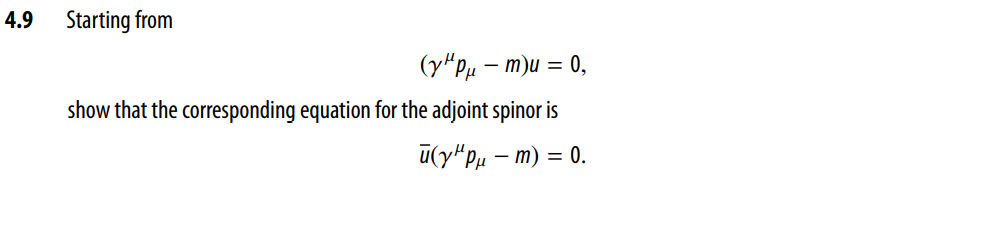
\includegraphics[scale = 0.55]{4.9a.png}
\end{figure}

We start with:

\begin{align}
    (\gamma^{\mu} p_{\mu} - m)u = 0
\end{align}

taking the Hermitian conjugate of each side, we get:

\begin{align}
    u^{\dagger}(\gamma^{\mu\dagger} p_{\mu} - m) = 0
\end{align}

we note we have shown before that:

\begin{align}
    (\gamma^{\mu})^{\dagger} = \gamma^{0} \gamma^{\mu} \gamma^{0}
\end{align}

thus our equation becomes:

\begin{align}
    u^{\dagger}(\gamma^{0} \gamma^{\mu} \gamma^{0} p_{\mu} - m) = 0
\end{align}

with $\gamma^{0} = 
\begin{pmatrix}
    1&0&0&0\\ 
    0&1&0&0\\ 
    0&0&-1&0\\ 
    0&0&0&-1
\end{pmatrix}$, we can show that:

\begin{align}
    \gamma^{0}\gamma^{0} &=
    \begin{pmatrix}
        1&0&0&0\\ 
        0&1&0&0\\ 
        0&0&-1&0\\ 
        0&0&0&-1
    \end{pmatrix}
    \begin{pmatrix}
        1&0&0&0\\ 
        0&1&0&0\\ 
        0&0&-1&0\\ 
        0&0&0&-1
    \end{pmatrix}\\
    &=
    \begin{pmatrix}
        1&0&0&0\\ 
        0&1&0&0\\ 
        0&0&1&0\\ 
        0&0&0&1
    \end{pmatrix}
    =I
\end{align}

thus we can manipulate our original equation as:

\begin{align}
    u^{\dagger}(\gamma^{0} \gamma^{\mu} \gamma^{0}\gamma^{0} p_{\mu} - m\gamma^{0}) &= 0\\
    u^{\dagger}(\gamma^{0} \gamma^{\mu} p_{\mu} - m\gamma^{0}) &= 0\\
\end{align}

by definition (Equation 4.36-4.37 of Thomson), $\bar{u} = u^{\dagger}\gamma^{0}$ so we can rewrite our equation as:

\begin{equation}\label{adjoint dirac}
\boxed{
    \bar{u}(\gamma^{\mu}p_{\mu} - m) = 0
}
\end{equation}


\begin{figure}[h!]
    \centering
    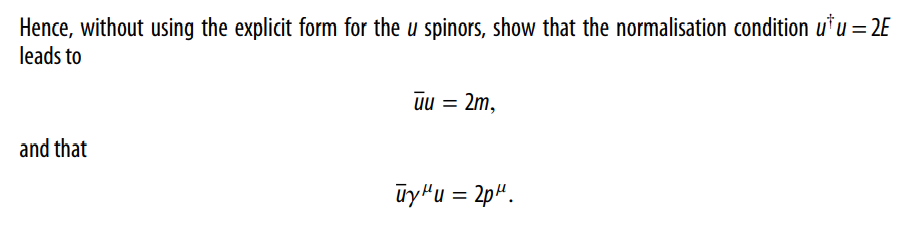
\includegraphics[scale = 0.55]{4.9b.png}
\end{figure}

We start with the original Dirac equation and the corresponding equation for the adjoint spinor:

\begin{align}
    (\gamma^{\mu} p_{\mu} - m)u &= 0\\
    \bar{u}(\gamma^{\mu}p_{\mu} - m) &= 0
\end{align}

since both equations zero out, we can manipulate each of them; by multiplying $\bar{u}\gamma^{\nu}$ by the first equation and multiplying the second equation by $\gamma^{\nu}u$:

\begin{align}
    \bar{u}\gamma^{\nu}[(\gamma^{\mu} p_{\mu} - m)u &= 0]\\
    [\bar{u}(\gamma^{\mu}p_{\mu} - m) &= 0]\gamma^{\nu}u
\end{align}

\begin{align}
    \bar{u}\gamma^{\nu}(\gamma^{\mu} p_{\mu} - m)u &= 0\\
    \bar{u}(\gamma^{\mu}p_{\mu} - m)\gamma^{\nu}u &= 0
\end{align}

adding these, we can get:

\begin{align}
    \bar{u}\gamma^{\nu}\gamma^{\mu}p_{\mu}u - \bar{u}\gamma^{\nu}um
    + \bar{u}\gamma^{\mu}\gamma^{\nu}p_{\mu}u - \bar{u}\gamma^{\nu}um = 0\\
    \bar{u}(\gamma^{\nu}\gamma^{\mu} + \gamma^{\mu}\gamma^{\nu})p_{\mu}u - 2\bar{u}\gamma^{\nu}um = 0
\end{align}

by Equation 4.33 of Thomson, we note of the anticommutation relation $\gamma^{\nu}\gamma^{\mu} + \gamma^{\mu}\gamma^{\nu} = 2g^{\mu\nu}$ and rewrite this as:

\begin{align}
    \bar{u}2g^{\mu\nu}p_{\mu}u - 2\bar{u}\gamma^{\nu}um = 0\\
    \bar{u}g^{\mu\nu}p_{\mu}u - \bar{u}\gamma^{\nu}um = 0
\end{align}

having the contravariant metric tensor $g^{\mu\nu}$ act on $p_{\mu}$ switches and raises its index, thus we have:

\begin{align}\label{case}
    \bar{u}p^{\nu}u - \bar{u}\gamma^{\nu}um = 0
\end{align}

now for the case of Equation \ref{case} of $\nu=0$, we have:

\begin{align}
    \bar{u}p^{0}u - \bar{u}\gamma^{0}um = 0
\end{align}

again using Equation 4.36-4.37 of Thomson, $\bar{u} = u^{\dagger}\gamma^{0}$, and noting that $p^0 = E$, then we have:

\begin{align}
    \bar{u}Eu - u^{\dagger}\gamma^{0}\gamma^{0}um = 0
\end{align}

with $\gamma^0\gamma^0=I$ and the given normalisation condition $u^{\dagger}u=2E$, then we get:

\begin{align}
    \bar{u}Eu - u^{\dagger}um = 0\\
    \bar{u}Eu = 2Em 
\end{align}

we finally arrive at:

\begin{equation}\label{newdef}
\boxed{
    \bar{u}u = 2m
}
\end{equation}

we can use Equation \ref{newdef} for the case of Equation \ref{case} where $\nu \neq 0$:

\begin{align}
    \bar{u}p^{\nu}u - \bar{u}\gamma^{\nu}um = 0\\
    2mp^{\nu} = \bar{u}\gamma^{\nu}um 
\end{align}

changing indices from $\nu$ to $\mu$ we then arrive at:

\begin{equation}
\boxed{
    \bar{u}\gamma^{\mu}u = 2p^{\mu}
}
\end{equation}

%we note that in our earlier solution evaluating $\gamma^{0}\gamma^{0}\gamma^{0}$, we found that $\gamma^{0}\gamma^{0} = \begin{pmatrix}1&0&0&0\\ 0&1&0&0\\ 0&0&1&0\\ 0&0&0&1\end{pmatrix} = I$. Thus we can rewrite the LHS of the equation as:

%\begin{align*}
%    -\gamma^{k} = -I\gamma^{k}\\
%    -\gamma^{k} = -\gamma^{0}\gamma^{0}\gamma^{k}
%\end{align*}

%we can rewrite the RHS of the equation as:

%\begin{align*}
%    \gamma^{0}\gamma^{k}\gamma^{0} = 
%\end{align*}
%==================================
\end{document}